\section{Method}
\label{methods}

Our self-training approach assumes access to a base language model, a small amount of seed data, and a collection of unlabelled examples, e.g. a web corpus. The unlabelled data is a large, diverse set of human-written documents which includes writing about all manner of topics humans are interested in -- but crucially is not paired with instructions. 
A \textbf{first key assumption} is that there exists some subset of this very large human-written text that would be suitable as gold generations for some user instructions.
A \textbf{second key assumption} is that we can predict  instructions for these candidate gold answers that can be used as high quality example pairs to train an instruction following model.


Our overall process,  which we call instruction backtranslation, 
 thus performs two core steps: 
\begin{enumerate}[leftmargin=*]
    \item {\em Self-augment}: Generate instructions for unlabelled data, i.e. the web corpus, to produce candidate training data of (instruction, output) pairs for instruction tuning. 
    \item {\em Self-curate}: Self-select high quality demonstration examples as training data to finetune the base model to follow instructions. This approach is done iteratively where a better intermediate instruction-following model can improve on selecting data for finetuning in the next iteration.
\end{enumerate}

We describe these steps in more details below. An overview of the approach is illustrated in \autoref{fig:method}.
\begin{figure}
  \centering
  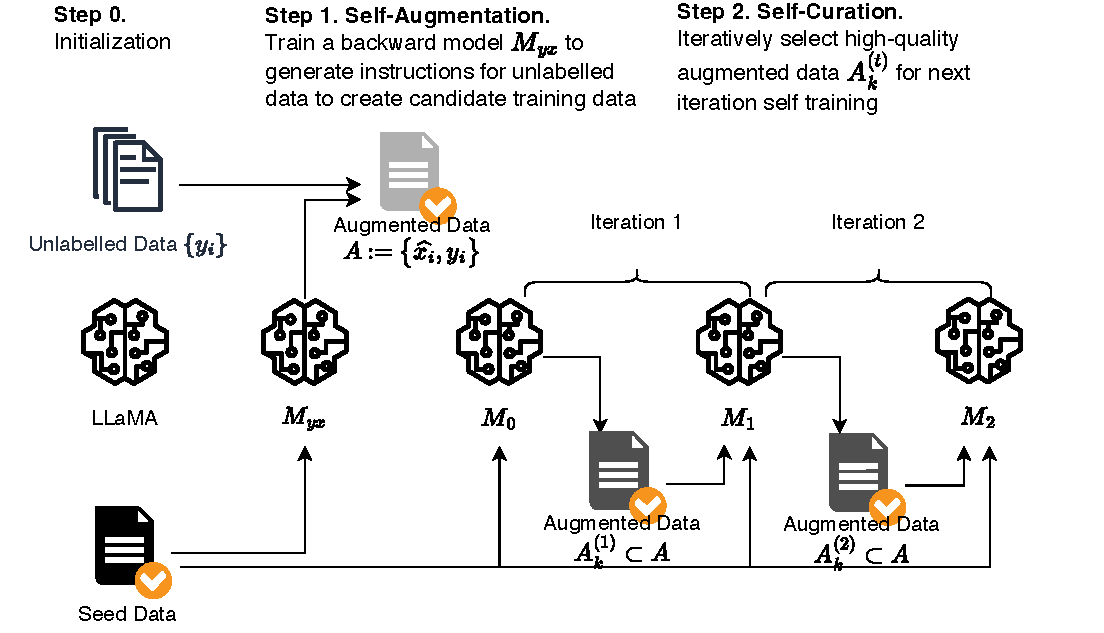
\includegraphics[width=1.0\columnwidth]{figs/fuzzy_v3.pdf}
  \caption{An overview of our {\bf instruction backtranslation} method. We start from a base language model, e.g. LLaMa, a small amount of seed examples of (instruction, output) pairs, and a collection of unlabelled documents which are considered candidate outputs for unknown instructions. \textbf{Self-augmentation}: the base model is finetuned with (output, instruction) pairs from the seed examples as an instruction prediction model
  $M_{yx}$, which is used to generate candidate instructions for outputs from the unlabelled data. \textbf{Self-curation}: starting from an intermediate instruction-following model $M_0$ finetuned from seed examples only, it selects high-quality (instruction, output) pairs $\mathcal{A}_k^{(1)}$ from the candidates from the previous step, and uses them as finetuning data for the next intermediate model $M_1$, which is in turn used to select training data for obtaining $M_2$. }
  \label{fig:method}
\end{figure}
\vspace{-3mm}

\subsection{Initialization}
\paragraph{Seed data.} We start with a seed set of human-annotated (instruction, output) examples that will be used to fine-tune language models to give initial predictions in both directions: predicting an output given an instruction, and an instruction given an output. 

\paragraph{Unlabelled data.} We use a web corpus as a source of unlabelled data.
For each document, we perform preprocessing to extract self-contained segments $\{ y_{i}\}$, which are portions of text following an HTML header. We further run deduplication, length filtering, and remove potential low quality segments with several heuristics such as the proportion of capitalized letters in the header. 


\subsection{Self-Augmentation (generating instructions)}  \label{sec:self-augment}

We finetune the base language model with (output, instruction) pairs $\{(y_{i}, x_{i})\}$ from the seed data to obtain a backward model $M_{yx}\coloneqq p(x|y)$. For each unlabelled example $y_i$, we run inference on the backward model to generate a candidate instruction $\hat{x_{i}}$ from which we  derive the  candidate augmented paired data $\mathcal{A} \coloneqq \{(\hat{x_{i}}, y_{i})\}$.
As we will see in experiments, not all of these candidate pairs are of high quality, and in that case using them all for self-training may not be beneficial. We thus consider the important next step of curation of a high quality subset.


\subsection{Self-Curation (selecting high-quality examples)} 

We select high quality examples using the language model itself. 
We start with a seed instruction model $M_{0}$ finetuned on (instruction, output) seed examples only. We then use $M_{0}$ to score each augmented example $\{(\hat{x}_{i}, y_{i})\}$ to derive a quality score $a_i$.  This is done using prompting, instructing the trained model to rate the quality of a candidate pair on a 5-point scale. The precise prompt we use is given in \autoref{table:rating_prompt}.
We can then select a subset of the augmented examples with score $a_i \ge k$ to form a curated set $\mathcal{A}_k^{(1)}$.

\paragraph{Iterative self-curation} 
We further propose an iterative training method to produce higher quality predictions.
On iteration $t$ we use the curated augmentation data $\mathcal{A}_k^{(t-1)}$ from the previous iteration, along with the seed data as training data to finetune an improved model $M_t$. This model in turn can be used to rescore the augmented examples for quality, resulting in an augmentation set $\mathcal{A}_k^{(t)}$. We perform two iterations of data selection and finetuning to get the final model $M_2$. 

When combining both seed data and augmented data for finetuning, we use tagging to distinguish these two data sources. Specifically, we append an additional sentence to examples (called ``system prompt"). We use $S_a \coloneqq$ ``Answer in the style of an AI Assistant." for seed data, and $S_w \coloneqq$ ``Answer with knowledge from web search." for augmented data. This approach is similar to methods used to tag synthetic data for backtranslation in machine translation \citep{caswell2019tagged}.

